\documentclass[11pt]{article}
\usepackage[a4paper,margin=27mm]{geometry}
\usepackage{mathptmx}
\usepackage{amsmath,amssymb,amsthm}
\usepackage{booktabs}
\usepackage{graphicx}
\usepackage{url}
\usepackage{algorithm}
\usepackage{algpseudocode}
\newcommand{\seg}[2]{\overline{#1\,#2}}

\newtheorem{theorem}{Theorem}
\newtheorem{propo}{Proposition}
\newtheorem{lemma}{Lemma}
\newtheorem{corollary}{Corollary}
\theoremstyle{definition}
\newtheorem{example}{Example}
\newtheorem{remark}{Remark}

\newcommand{\U}{\mathbf{U}}
\newcommand{\R}{\mathbb{R}}
\newcommand{\eps}{\varepsilon}
\newcommand{\ex}{\eps_x}
\newcommand{\ey}{\eps_y}
\newcommand{\rng}{\operatorname{rng}}
\newcommand{\wid}{\operatorname{wid}}
\newcommand{\mmid}{\operatorname{mid}}

\title{Exact multiplication of reduced affine forms}
\author{Ignacio Araya$^{1,*}$, Daniel Miranda$^{1}$, Victor Reyes$^{2}$, Juan Geraldo$^{1}$\\[2mm]
\small $^{1}$Escuela de Ingenier\'{\i}a Inform\'atica, Pontificia Universidad Cat\'olica de Valpara\'{\i}so, Valpara\'{\i}so, Chile\\
\small $^{2}$Facultad de Ingenier\'{\i}a y Ciencias, Universidad Diego Portales, Santiago, Chile\\[1mm]
\small \texttt{ignacio.araya@pucv.cl}, \texttt{daniel.miranda.v@mail.pucv.cl},\\ \small \texttt{victor.reyes1@mail.udp.cl}, \texttt{juan.geraldo.u@mail.pucv.cl}\\[1mm]
\small ORCID: I.~Araya 0000-0001-5882-6217, V.~Reyes 0000-0002-3358-3906\\[1mm]
\small $^{*}$Corresponding author}
\date{}

\begin{document}
\maketitle

\begin{abstract}
Reduced affine forms keep a fixed number of noise symbols and accumulate all the approximation errors in a single error term. The product of two such forms must be enclosed by a new reduced affine form, and the width of this enclosure determines the quality of range bounds and of the linear relaxations built from the forms in branch-and-bound solvers. Skalna and Hlad\'{\i}k computed in linear time the exact range of the quadratic part of the product. We show that their multiplication is not exact in general when both operands carry errors, because the terms that couple the centers of the operands with their error symbols are bounded separately, and we give a multiplication that computes the exact range of the whole nonlinear part of the product in $O(n\log n)$ time, by a single walk along the boundary of a planar zonotope. We prove that it coincides with that of Skalna and Hlad\'{\i}k when one operand has no error or a zero center, and that it is at most $3/2$ times narrower otherwise, a tight bound. We also give a rigorous floating-point implementation of both multiplications. In an interval branch-and-bound optimizer, replacing the standard multiplication used by default by either of them reduces the number of nodes about four times on problems dominated by products; the new multiplication saves a further 4--8\% of the nodes precisely on the problems where the theory predicts a gain, and coincides with that of Skalna and Hlad\'{\i}k elsewhere.

\medskip\noindent
\textit{Keywords:} reduced affine arithmetic, multiplication, range enclosure, linear relaxation, zonotope
\end{abstract}

\section{Introduction}

Affine arithmetic (AA)~\cite{combastolfi1993,stolfi1997self,defigueiredo2004affine} represents an uncertain quantity by an affine function of noise symbols $\eps_i\in\U=[-1,1]$, and keeps the linear dependencies between quantities that share symbols. Each nonlinear operation of standard AA introduces a new symbol, so the forms grow along long computations. Reduced affine forms~\cite{messine2002extentions,vu2009enhancing,skalna2017new} keep only the $n$ symbols of the initial uncertain parameters and accumulate all the errors in one term,
\begin{equation}
\label{eq:raf}
\hat x = x_0 + \sum_{i=1}^n x_i\eps_i + x_r\ex,\qquad x_r\ge 0,\ \ex\in\U .
\end{equation}
They are the basis of the reliable affine relaxations used in interval branch-and-bound solvers~\cite{ninin2015reliable}: over a box, each $\eps_i$ is an affine function of the variable $x_i$, so that a form is a linear function of the variables plus an interval, and its two bounding hyperplanes are a range enclosure and a linear relaxation of the corresponding expression. The vertical distance between them, $2x_r$, measures the quality of the relaxation.

The product of two reduced affine forms is a quadratic function of the symbols and must be enclosed by a new reduced affine form. The multiplications proposed in the literature keep the same linear part and differ in how they enclose the remaining nonlinear terms, which consist of the quadratic part $(e^Tx+x_r\ex)(e^Ty+y_r\ey)$ and of the terms $x_0y_r\ey+y_0x_r\ex$ that couple the center of each operand with the error of the other (Section~\ref{sec:products}):
\begin{itemize}
\item The \emph{trivial} multiplication of standard AA~\cite{stolfi1997self} bounds the quadratic part by the product of the total radii of the operands, $(\|x\|_1+x_r)(\|y\|_1+y_r)$, as if all its terms could reach their largest absolute values at the same time.
\item The \emph{standard} multiplication~\cite{kolev2004improved,vu2009enhancing} uses that the squares $\eps_i^2$ range over $[0,1]$ instead of $[-1,1]$: it moves the center by $\tfrac12x^Ty$ and removes $\tfrac12|x|^T|y|$ from the radius. AF2~\cite{messine2002extentions} exploits the same fact differently, by keeping two one-sided error terms for the positive and the negative squares.
\item A formula attributed to Miyajima~\cite{skalna2017new} also groups the two bilinear terms $x_iy_j\eps_i\eps_j$ and $x_jy_i\eps_j\eps_i$ of each pair before bounding them, which helps when they cancel.
\item The \emph{best multiplication} of Miyajima, Miyata and Kashiwagi~\cite{miyajima2003best}, implemented in the kv library~\cite{kvlib}, computes the exact range of the whole quadratic part, including the error symbols of the operands, in $O(n^2)$ time.
\item Skalna and Hlad\'{\i}k~\cite{skalna2017new} compute the same exact range in linear time. They observe that $(e^Tx,e^Ty)$ ranges over a planar zonotope, whose boundary is described by the generators $(x_i,y_i)$ sorted by angle, and that the product $uv$ attains its extrema on that boundary. They describe their multiplication as yielding the minimum Chebyshev-type bounds, and it is the tightest of the existing formulae.
\end{itemize}
The best multiplication and the multiplication of Skalna and Hlad\'{\i}k stop at the quadratic part because in standard AA it is all that has to be bounded: the terms $x_0(\hat y-y_0)+y_0(\hat x-x_0)$ stay as linear terms in their own symbols, and Rump and Kashiwagi~\cite{rump2015implementation} refer to~\cite{miyajima2003best} for the optimal bound of the quadratic part. In reduced affine forms, however, the terms $x_0y_r\ey+y_0x_r\ex$ involve the error symbols of the operands and must be folded into the new error term, and both the kv implementation for forms with an accumulated error term and the multiplication of Skalna and Hlad\'{\i}k add their bound $|y_0|x_r+|x_0|y_r$ separately.

In this paper we observe that the multiplication of Skalna and Hlad\'{\i}k is not exact in general when both operands carry errors: two terms of the product, $x_0 y_r\ey$ and $y_0 x_r\ex$, are bounded separately from the quadratic part, although they share the error symbols with it. We show that the whole nonlinear part of the product is affine in each of the two error symbols, so that its range is the union of four ranges obtained with the error symbols fixed at the vertices of $\U^2$; for each vertex, what remains is a product of two shifted linear functions of the symbols, whose exact range follows from the geometry of planar zonotopes used by Skalna and Hlad\'{\i}k, and, by the central symmetry of the zonotope, opposite vertices give the same range up to a constant, so that two ranges suffice. The resulting multiplication computes the exact range of the nonlinear part of the product, in $O(n\log n)$ time.

\paragraph{Contributions.}
\begin{itemize}
\item An exact multiplication of reduced affine forms, E (Section~\ref{sec:exact}): Theorem~\ref{thm:exact} shows that it gives the narrowest enclosure of the product with the usual linear part, and Algorithm~\ref{alg:exact} computes it in $O(n\log n)$ time.
\item Its relation with the existing formulae (Section~\ref{sec:hierarchy}): E is contained in the multiplication SH of Skalna and Hlad\'{\i}k, which is contained in the standard and trivial ones; E coincides with SH when one operand has no error (Proposition~\ref{prop:oneerror}) and is at most $3/2$ times narrower otherwise, a tight bound (Proposition~\ref{prop:32}); the difference of widths is at most $2\min(|x_0|y_r,|y_0|x_r)$, and usually equal to it, so that E can only help when both operands carry errors and have nonzero centers (Corollary~\ref{cor:gain}). We also show that the standard multiplication is AF2~\cite{messine2002extentions} with its one-sided error terms re-centered after each product (Proposition~\ref{prop:af2}).
\item A rigorous floating-point implementation of SH and E (Section~\ref{sec:rigor}), with an exact angular predicate and an a priori bound of the rounding errors of the boundary walk.
\item Experiments (Section~\ref{sec:experiments}) on range enclosures, with exact ranges computed by a global optimizer, and in an interval global optimizer, where SH and E reduce the search tree about four times on problems dominated by products, and E improves on SH precisely where Corollary~\ref{cor:gain} predicts.
\end{itemize}

\section{Products of reduced affine forms}
\label{sec:products}

Let $\hat x$ be as in~\eqref{eq:raf} and $\hat y = y_0+\sum_i y_i\eps_i + y_r\ey$, and write $x=(x_1,\dots,x_n)$, $y=(y_1,\dots,y_n)$ and $e=(\eps_1,\dots,\eps_n)\in\U^n$. Following~\cite{skalna2017new},
\begin{equation}
\label{eq:product}
\hat x\hat y = x_0y_0 + e^T(y_0x+x_0y) + N(e,\ex,\ey),
\end{equation}
\begin{equation}
\label{eq:N}
N(e,\ex,\ey) = x_0y_r\ey + y_0x_r\ex + (e^Tx + x_r\ex)(e^Ty + y_r\ey).
\end{equation}
All the formulae considered here keep the linear part $x_0y_0+e^T(y_0x+x_0y)$ and enclose $N$ over $\U^{n+2}$ by an interval $[c-z_r,\,c+z_r]$, which gives the reduced affine form
\begin{equation}
\label{eq:zhat}
\hat z = x_0y_0 + c + e^T(y_0x+x_0y) + z_r\eps_z .
\end{equation}
A multiplication formula is therefore an enclosure of $\rng N$, the range of $N$ over $\U^{n+2}$, and its quality is the width $2z_r$, the thickness of the resulting relaxation. Denote $\|x\|_1=\sum_i|x_i|$, $|x|=(|x_1|,\dots,|x_n|)$, and
\[
R(e,\ex,\ey) = (e^Tx + x_r\ex)(e^Ty + y_r\ey), \qquad Q(e) = (e^Tx)(e^Ty) = \sum_i x_iy_i\eps_i^2 + \sum_{i<j}(x_iy_j+x_jy_i)\eps_i\eps_j .
\]
We consider the following formulae, labeled as in~\cite{skalna2017new} when they appear there.
\begin{description}
\item[T, trivial~\cite{stolfi1997self} (Eq.~4 of~\cite{skalna2017new}).] $c=0$, $z_r = |y_0|x_r+|x_0|y_r+(\|x\|_1+x_r)(\|y\|_1+y_r)$.
\item[S, standard~\cite{kolev2004improved,vu2009enhancing} (Eq.~5).] $c=\tfrac12 x^Ty$, $z_r = |y_0|x_r+|x_0|y_r+(\|x\|_1+x_r)(\|y\|_1+y_r) - \tfrac12|x|^T|y|$. The squares $x_iy_i\eps_i^2\in x_iy_i[0,1]$ are enclosed by their exact range.
\item[SH, Skalna and Hlad\'{\i}k~\cite{skalna2017new} (Eq.~10).] $[c-z_r,c+z_r] = [R_{\min},R_{\max}] + [-1,1](|y_0|x_r+|x_0|y_r)$, where $[R_{\min},R_{\max}]=\rng R$ is computed exactly in $O(n)$ time. The best multiplication of~\cite{miyajima2003best}, as implemented in the kv library~\cite{kvlib} (option \texttt{AFFINE\_MULT=2}), gives the same interval, with an $O(n^2)$ algorithm.
\item[E, exact (this paper).] $[c-z_r,c+z_r]=\rng N$.
\end{description}
We say that a formula is \emph{exact} when its interval is the range of the whole nonlinear part, $\rng N$ (or $\rng N_2$ for a square): SH computes the exact range of the quadratic part $R$, and it is exact in this sense when one of the operands has no error or a zero center (Corollary~\ref{cor:gain}), but not in general, while E is always exact. The Chebyshev square is exact in the same sense when $x_r\le\|x\|_1$ (Proposition~\ref{prop:square}). Skalna and Hlad\'{\i}k also consider an intermediate formula attributed to Miyajima (Eq.~6 of~\cite{skalna2017new}), which groups the two bilinear terms $x_iy_j$ and $x_jy_i$ of each pair before bounding them; it lies between SH and S~\cite[Prop.~3]{skalna2017new} and plays no role in what follows.

\paragraph{Squares.} For the square $\hat x\hat x$ of a form, the two operands share the error symbol, and~\eqref{eq:product} becomes $\hat x^2=x_0^2+2x_0\,e^Tx+N_2(e,\ex)$, with nonlinear part
\begin{equation}
\label{eq:N2}
N_2(e,\ex)=2x_0x_r\ex+(e^Tx+x_r\ex)^2 ,
\end{equation}
which is $N$ with $\hat y=\hat x$ and $\ey=\ex$. The formulae above apply with $\ey=\ex$: S gives $c=\tfrac12x^Tx$ and $z_r=2|x_0|x_r+(\|x\|_1+x_r)^2-\tfrac12x^Tx$, and SH encloses the quadratic part by its exact range $[0,(\|x\|_1+x_r)^2]$ and adds $[-1,1]\,2|x_0|x_r$. Proposition~\ref{prop:square} gives the exact range of $N_2$ and shows that the latter is exact when $x_r\le\|x\|_1$.

\paragraph{AF2.} AF2~\cite{messine2002extentions} keeps, besides the symmetric error term, two one-sided error terms that record errors of known sign; its product is described in Section~\ref{sec:hierarchy}, where it is related to formula S.

\section{The exact multiplication}
\label{sec:exact}

\begin{lemma}
\label{lem:vertices}
$\min N = \min_{s,t\in\{-1,1\}}\ \min_{e\in\U^n} N(e,s,t)$ and $\max N = \max_{s,t\in\{-1,1\}}\ \max_{e\in\U^n} N(e,s,t)$, where $\min N$ and $\max N$ are taken over $\U^{n+2}$. Hence $\rng N$, which is an interval since $N$ is continuous and $\U^{n+2}$ is compact and connected, is determined by the four ranges $\rng_e N(\cdot,s,t)$ over $e\in\U^n$.
\end{lemma}
\begin{proof}
For fixed $e$, $N(e,\ex,\ey)$ is a bilinear function of $(\ex,\ey)$, by~\eqref{eq:N}: for fixed $\ey$ it is affine in $\ex$, so its extrema over $\ex\in\U$ are attained at $\ex=\pm1$, and for fixed $\ex=\pm1$ it is affine in $\ey$, so its extrema over $\ey\in\U$ are attained at $\ey=\pm1$. Hence its extrema over $\U^2$ are attained at vertices: for every $(e,\ex,\ey)\in\U^{n+2}$ there are $(s,t)$, $(s',t')\in\{-1,1\}^2$ with $N(e,s,t)\le N(e,\ex,\ey)\le N(e,s',t')$. The minimum and the maximum of $N$ are therefore attained with $(\ex,\ey)$ at a vertex of $\U^2$.
\end{proof}

For fixed $(s,t)$,
\begin{equation}
\label{eq:Nst}
N(e,s,t) = x_0y_rt+y_0x_rs + (u + x_rs)(v + y_rt),\qquad (u,v)=(e^Tx,\,e^Ty)\in Z,
\end{equation}
where $Z=\{\sum_i\eps_i(x_i,y_i): e\in\U^n\}\subset\R^2$ is the joint range of $e^Tx$ and $e^Ty$, a planar zonotope with generators $g_i=(x_i,y_i)$~\cite{ziegler1995lectures}. The range of~\eqref{eq:Nst} is thus $\kappa$ plus the range over $Z$ of the shifted product $\varphi_\delta(u,v)=(u+\delta_1)(v+\delta_2)$, where $\kappa=x_0y_rt+y_0x_rs$ and $\delta=(x_rs,\,y_rt)$; equivalently, of the product $\varphi_0(u,v)=uv$ over the translate $Z+\delta$.

\begin{lemma}
\label{lem:zonotope}
Let $Z$ be a planar zonotope and $\delta\in\R^2$. The minimum and the maximum of $\varphi_\delta$ over $Z$ are attained on the boundary of $Z$. If the nonzero generators are replaced by $\tilde g_i=\pm g_i$ so that they lie in the half-plane $\{u>0\}\cup\{u=0,v>0\}$ and are sorted by increasing angle, $\tilde g_{(1)},\dots,\tilde g_{(m)}$, the boundary of $Z$ is the polygon with vertices
\begin{equation}
\label{eq:boundary}
p_0=-\sum_k\tilde g_{(k)},\quad p_k = p_{k-1}+2\tilde g_{(k)}\ (k=1,\dots,m),\quad p_{m+k} = p_{m+k-1}-2\tilde g_{(k)}\ (k=1,\dots,m).
\end{equation}
\end{lemma}
\begin{proof}
The only critical point of $\varphi_\delta$ is $(-\delta_1,-\delta_2)$, where the Hessian $\left(\begin{smallmatrix}0&1\\1&0\end{smallmatrix}\right)$ is indefinite. A local extremum in the interior of $Z$ would be a critical point with a semidefinite Hessian, so there is none, and the extrema of the continuous function $\varphi_\delta$ on the compact set $Z$ lie on its boundary. Replacing $g_i$ by $-g_i$ does not change $Z$, since $\eps_i$ ranges over a symmetric interval. The description of the boundary of a planar zonotope by its generators sorted by angle is classical; see~\cite{ziegler1995lectures} and~\cite[Prop.~7]{skalna2017new} for the part of the boundary in the nonnegative quadrant.
\end{proof}

\begin{lemma}
\label{lem:pairs}
For $(s,t)\in\{-1,1\}^2$, let $\kappa_{st}=x_0y_rt+y_0x_rs$ and $[m_{st},M_{st}]$ be the range of $\varphi_\delta$ over $Z$ with $\delta=(x_rs,y_rt)$, so that $\rng_eN(\cdot,s,t)=\kappa_{st}+[m_{st},M_{st}]$ by~\eqref{eq:Nst}. Then $[m_{-s,-t},M_{-s,-t}]=[m_{st},M_{st}]$ and $\kappa_{-s,-t}=-\kappa_{st}$; hence
\[
\rng N=\Big[\min_{t\in\{-1,1\}}\big(m_{1t}-|\kappa_{1t}|\big),\ \max_{t\in\{-1,1\}}\big(M_{1t}+|\kappa_{1t}|\big)\Big].
\]
\end{lemma}
\begin{proof}
Since $Z=-Z$ and $\varphi_{-\delta}(-u,-v)=(-u-\delta_1)(-v-\delta_2)=\varphi_\delta(u,v)$, the function $\varphi_{-\delta}$ takes on $Z$ the same values as $\varphi_\delta$. The opposite vertices $(s,t)$ and $(-s,-t)$ therefore contribute $\kappa_{st}+[m_{st},M_{st}]$ and $-\kappa_{st}+[m_{st},M_{st}]$, whose union has extreme values $m_{st}-|\kappa_{st}|$ and $M_{st}+|\kappa_{st}|$, and Lemma~\ref{lem:vertices} gives the result.
\end{proof}

\begin{figure}[t]
\centering
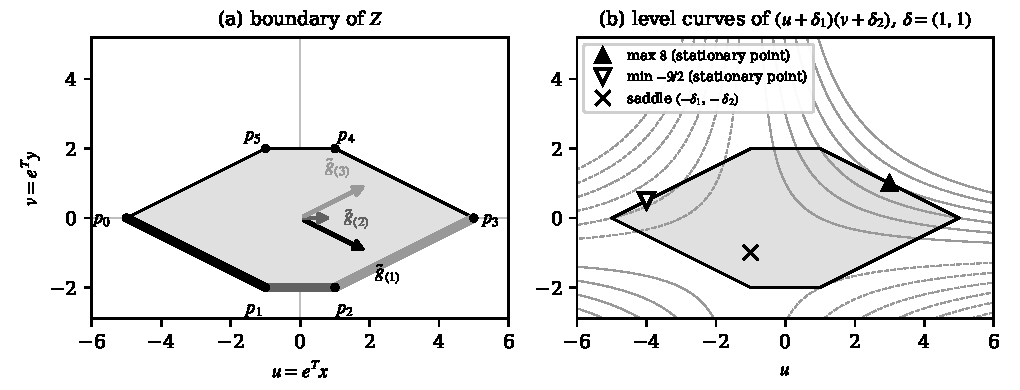
\includegraphics[width=\linewidth]{Fig1.pdf}
\caption{Lemma~\ref{lem:zonotope} and Algorithm~\ref{alg:exact} on Example~\ref{ex:alg}. (a) The generators $(2,-1)$, $(1,0)$, $(2,1)$, turned to the half-plane $u>0$ and sorted by angle; the boundary of $Z$ starts at $p_0=-\sigma$, adds $2\tilde g_{(1)},2\tilde g_{(2)},2\tilde g_{(3)}$ (thick edges, in three shades of gray like the generators) and then subtracts them in the same order. (b) Level curves of $\varphi_\delta$ for $\delta=(1,1)$, the vertex $(s,t)=(1,1)$ (dashed: negative values); the maximum and the minimum over $Z$ are marked with a black and a white triangle. Its only critical point is a saddle, so its extrema over $Z$ lie on the boundary; here both are attained at stationary points of edges. Algorithm~\ref{alg:exact} performs this walk, in a single pass, for the two shifts $\delta=(x_r,\pm y_r)$ (Lemma~\ref{lem:pairs}).}
\label{fig:zonotope}
\end{figure}

Let the segment $\seg pq$ be an edge of the translated polygon $Z+\delta$ and let $d=q-p$, so that the points of the edge are $p+\tau d$, $\tau\in[0,1]$. Then
\[
\varphi_0(p+\tau d)=(p_u+\tau d_u)(p_v+\tau d_v)=P+B\tau+A\tau^2,\qquad P=p_up_v,\ B=p_ud_v+p_vd_u,\ A=d_ud_v,
\]
whose extrema over $[0,1]$ are attained at $\tau\in\{0,1\}$, with values $\varphi_0(p)$ and $\varphi_0(q)$, or, if $A\ne0$ and $\tau^*=-B/(2A)\in(0,1)$, at the stationary point, with value $P-B^2/(4A)$. This gives Algorithm~\ref{alg:exact}.

\begin{algorithm}[t]
\caption{Exact multiplication of reduced affine forms}
\label{alg:exact}
\begin{algorithmic}[1]
\Require $\hat x = x_0+\sum_ix_i\eps_i+x_r\ex$, $\hat y = y_0+\sum_iy_i\eps_i+y_r\ey$
\Ensure $\hat z$ with $\hat x\hat y\in\hat z$ for all $e,\ex,\ey$, and $x_0y_0+c\pm z_r = x_0y_0+\rng N$
\State $\tilde g_{(1)},\dots,\tilde g_{(m)}\gets$ the nonzero $(x_i,y_i)$, turned to the half-plane $u>0$ and sorted by angle
\State $\delta^{(1)}\gets(x_r,y_r)$, $\delta^{(2)}\gets(x_r,-y_r)$;\quad $\kappa_1\gets|x_0y_r+y_0x_r|$, $\kappa_2\gets|x_0y_r-y_0x_r|$
\State $\ell_k\gets+\infty$, $h_k\gets-\infty$ ($k=1,2$);\quad $p\gets-\sum_{k=1}^m\tilde g_{(k)}$ \Comment{vertex $p_0$ of~\eqref{eq:boundary}}
\For{$j=1,\dots,2m$}
  \State $d\gets2\tilde g_{(j)}$ if $j\le m$, and $d\gets-2\tilde g_{(j-m)}$ otherwise
  \For{$k=1,2$} \Comment{the edge $\seg{p}{(p+d)}$, translated by $\delta^{(k)}$}
    \State $a\gets p+\delta^{(k)}$, $b\gets a+d$
    \State $\ell_k\gets\min(\ell_k,\,b_ub_v)$, $h_k\gets\max(h_k,\,b_ub_v)$
    \State $A\gets d_ud_v$, $B\gets a_ud_v+a_vd_u$
    \If{$A\ne0$ and $0<-B/(2A)<1$}
      \State $w\gets a_ua_v-B^2/(4A)$
      \State $\ell_k\gets\min(\ell_k,w)$, $h_k\gets\max(h_k,w)$
    \EndIf
  \EndFor
  \State $p\gets p+d$
\EndFor
\State $\ell\gets\min(\ell_1-\kappa_1,\,\ell_2-\kappa_2)$, $h\gets\max(h_1+\kappa_1,\,h_2+\kappa_2)$
\State $c\gets(\ell+h)/2$, $z_r\gets(h-\ell)/2$ (rounded outwards in a rigorous implementation)
\State \Return $\hat z = x_0y_0+c+e^T(y_0x+x_0y)+z_r\eps_z$
\end{algorithmic}
\end{algorithm}

Algorithm~\ref{alg:exact} works as follows (Figure~\ref{fig:zonotope}). Line~1 turns the generators to the half-plane $u>0$ and sorts them by angle. By Lemma~\ref{lem:pairs}, only the vertices $(1,1)$ and $(1,-1)$ of $\U^2$ are needed, with shifts $\delta^{(1)}$, $\delta^{(2)}$ and constants of absolute values $\kappa_1$, $\kappa_2$ (line~2). The two translated polygons $Z+\delta^{(k)}$ have the same edges, so a single walk visits both: it starts at the vertex $p_0$ of~\eqref{eq:boundary} and follows it, adding the edge vectors $2\tilde g_{(1)},\dots,2\tilde g_{(m)}$ and then subtracting them in the same order, so that $p$ visits all the vertices of $Z$ and returns to the start. For each edge and each shift, the algorithm evaluates $\varphi_0$ at the end $b$ of the translated edge and, if it lies inside the edge, at the stationary point, which is a maximum of $\varphi_0$ on the edge when $A<0$ and a minimum when $A>0$ (updating both $\ell_k$ and $h_k$ with it is harmless); since the polygon is closed, the ends of the $2m$ edges are all its vertices, including the starting one, which is the end of the last edge. After the walk, $[\ell_k,h_k]$ is the range of $\varphi_0$ over $Z+\delta^{(k)}$, line~17 applies Lemma~\ref{lem:pairs}, and the midpoint and half-width of $[\ell,h]=\rng N$ give the new center shift $c$ and error term $z_r$. (If $m=0$, $Z=\{0\}$, and $\ell_k=h_k=\delta^{(k)}_1\delta^{(k)}_2$.)

\begin{theorem}
\label{thm:exact}
Algorithm~\ref{alg:exact} computes $\rng N$ exactly (in exact arithmetic) in $O(n\log n)$ time. Consequently, among all reduced affine forms with linear part $e^T(y_0x+x_0y)$ that enclose $\hat x\hat y$ over $\U^{n+2}$, the one returned by Algorithm~\ref{alg:exact} has the smallest error term $z_r$.
\end{theorem}
\begin{proof}
By Lemma~\ref{lem:pairs}, $\rng N$ is determined by the ranges of $\varphi_\delta$ over $Z$ for the shifts $\delta^{(1)}$ and $\delta^{(2)}$, and by Lemma~\ref{lem:zonotope} each of them is the range of $\varphi_0$ over the boundary of $Z+\delta^{(k)}$, which the walk computes exactly. The generators are sorted once, in $O(n\log n)$ time, and the walk along the $2m\le 2n$ edges, with two shifts, takes $O(n)$ time. For the second statement, a reduced affine form with that linear part encloses $\hat x\hat y$ if and only if $[c-z_r,c+z_r]\supseteq\rng N$, by~\eqref{eq:product}; the narrowest such interval is $\rng N$.
\end{proof}

\begin{example}
\label{ex:alg}
Let $\hat x=1+\eps_1+2\eps_2+2\eps_3+\ex$ and $\hat y=1+\eps_2-\eps_3+\ey$, so that $n=3$ and $x_r=y_r=1$. The generators $(1,0)$, $(2,1)$ and $(2,-1)$ already lie in the half-plane $u>0$; sorted by angle, $\tilde g_{(1)}=(2,-1)$, $\tilde g_{(2)}=(1,0)$ and $\tilde g_{(3)}=(2,1)$, so $\sigma=(5,0)$ and $Z$ is the hexagon with vertices $(-5,0)$, $(-1,-2)$, $(1,-2)$, $(5,0)$, $(1,2)$, $(-1,2)$ (Figure~\ref{fig:zonotope}a). The shifts are $\delta^{(1)}=(1,1)$ and $\delta^{(2)}=(1,-1)$, with $\kappa_1=2$ and $\kappa_2=0$. For $\delta^{(1)}$, for instance, the walk starts at $p_0+\delta^{(1)}=(-4,1)$, and on the fourth edge, from $p=(6,1)$ to $q=(2,3)$ with $d=(-4,2)$, $\varphi_0(p+\tau d)=6+8\tau-8\tau^2$ reaches its maximum $8$ at $\tau^*=\tfrac12$, the point $(4,2)$, although it is $6$ at both ends of the edge. The walk gives the following extrema of $uv$ over the two translated hexagons; in this example all of them are attained at stationary points of edges, at $\tau^*\in\{\tfrac14,\tfrac12,\tfrac34\}$:
\begin{center}
\small
\begin{tabular}{rrrrr}
\toprule
$\delta^{(k)}$ & $\kappa_k$ & $\ell_k=\min uv$ & $h_k=\max uv$ & $[\ell_k-\kappa_k,\,h_k+\kappa_k]$ \\
\midrule
$(1,1)$ & $2$ & $-\tfrac92$ & $8$ & $[-\tfrac{13}2,10]$ \\
$(1,-1)$ & $0$ & $-8$ & $\tfrac92$ & $[-8,\tfrac92]$ \\
\bottomrule
\end{tabular}
\end{center}
Hence $\rng N=[-8,10]$, $c=1$, $z_r=9$, and, with the linear part $x_0y_0+e^T(y_0x+x_0y)=1+\eps_1+3\eps_2+\eps_3$, Algorithm~\ref{alg:exact} returns $\hat z=2+\eps_1+3\eps_2+\eps_3+9\eps_z$. The multiplication of Skalna and Hlad\'{\i}k encloses $R$ by its exact range $[-8,8]$ and adds $\pm(|y_0|x_r+|x_0|y_r)=\pm2$, which gives $[-10,10]$ and $z_r=10$. Here $2\min(|x_0|y_r,|y_0|x_r)=2$ is exactly the difference of widths, the largest one allowed by Corollary~\ref{cor:gain}.
\end{example}

\begin{remark}
Skalna and Hlad\'{\i}k compute $R_{\max}$ in linear time by replacing the sorting with repeated median selection~\cite[Prop.~8]{skalna2017new}, using the central symmetry of $\varphi_0$. The shifted products $\varphi_\delta$ lack this symmetry, and we leave a linear-time version of Algorithm~\ref{alg:exact} open; for moderate $n$, the $O(n\log n)$ version is the one recommended in~\cite{skalna2017new}.
\end{remark}

\begin{remark}
When $x_r=y_r=0$, $N=Q$ and E gives the exact range of $\hat x\hat y - x_0y_0 - e^T(y_0x+x_0y)$; over a box, this is the narrowest residual of a linear relaxation of the product of two affine functions with the given slopes. All the multiplication formulae of Section~\ref{sec:products} keep the linear part~\eqref{eq:product}; choosing another linear part, as in the min-range approximations of~\cite{stolfi1997self,skalna2013minrange}, is a different problem that we do not consider.
\end{remark}

\section{A hierarchy of multiplication formulae}
\label{sec:hierarchy}

Denote by $[\hat z]_F$ the interval $[c-z_r,c+z_r]$ of formula $F$.

\begin{propo}
\label{prop:chain}
For all operands, $[\hat z]_E \subseteq [\hat z]_{SH}\subseteq[\hat z]_S\subseteq[\hat z]_T$.
\end{propo}
\begin{proof}
$[\hat z]_E=\rng N$ is contained in every valid enclosure. The inclusions $[\hat z]_{SH}\subseteq[\hat z]_S\subseteq[\hat z]_T$ follow from~\cite[Prop.~3]{skalna2017new}. The first one holds because the part of $[\hat z]_S$ that does not come from $|y_0|x_r+|x_0|y_r$ is a valid enclosure of $R$, which SH replaces by its exact range, and the second because the radius of S is that of T minus $\tfrac12|x|^T|y|$ and its center moves by $\tfrac12x^Ty$, with $|\tfrac12x^Ty|\le\tfrac12|x|^T|y|$. We will also use the identity
\[
(\|x\|_1+x_r)(\|y\|_1+y_r) - \tfrac12|x|^T|y| = \tfrac12|x|^T|y|+\sum_{i\ne j}|x_iy_j| + x_r\|y\|_1+y_r\|x\|_1+x_ry_r .
\]
\end{proof}

The difference between E and SH comes from the terms $x_0y_r\ey$ and $y_0x_r\ex$, which SH bounds separately. When one of the operands has no error, this separation costs nothing.

\begin{propo}
\label{prop:oneerror}
If $x_r=0$ or $y_r=0$, then $[\hat z]_E=[\hat z]_{SH}$.
\end{propo}
\begin{proof}
Let $y_r=0$, so that $N = y_0x_r\ex + R$ with $R(e,\ex)=(e^Tx+x_r\ex)\,e^Ty$. Since $R$ is affine in $\ex$ for fixed $e$, its maximum over $\U^{n+1}$ is attained at some $(e^*,\ex^*)$ with $\ex^*\in\{-1,1\}$, and since $R(-e,-\ex)=R(e,\ex)$, also at $(-e^*,-\ex^*)$. Choosing the one with $\ex^*=\operatorname{sign}(y_0)$ (either, if $y_0=0$) gives $N = |y_0|x_r + R_{\max}$, which is the upper bound of $[\hat z]_{SH}$. The same argument applies to the lower bound, and to $x_r=0$.
\end{proof}

When both operands carry errors, E can be narrower than SH, but by a bounded factor. Denote $A=|y_0|x_r+|x_0|y_r$ and, for the two pairs of opposite vertices of $\U^2$, $\Lambda_\alpha=|x_0y_r+y_0x_r|$, the value of $|x_0y_r\ey+y_0x_r\ex|$ at $(\ex,\ey)=\pm(1,1)$, and $\Lambda_\beta=|x_0y_r-y_0x_r|$, its value at $\pm(1,-1)$, so that $\max(\Lambda_\alpha,\Lambda_\beta)=A$; these are the constants $\kappa_1$ and $\kappa_2$ of Algorithm~\ref{alg:exact}.

\begin{lemma}
\label{lem:classes}
The maximum of $R$ over $\U^{n+2}$ is attained at a point with $(\ex,\ey)=(1,1)$, and its minimum at a point with $(\ex,\ey)=(1,-1)$.
\end{lemma}
\begin{proof}
Write $R=(u+x_r\ex)(v+y_r\ey)$ with $(u,v)=(e^Tx,e^Ty)$. Since $R(0,0,0)=0$, $\max R\ge0$. If $\max R=0$, it is attained at $(e,\ex,\ey)=(0,1,1)$, where $R=x_ry_r\ge0$. Otherwise, at a maximizer both factors have the same sign, and since $R(-e,-\ex,-\ey)=R(e,\ex,\ey)$, we may assume, replacing the maximizer by its opposite if necessary, that both are positive. Increasing $\ex$ and $\ey$ to $1$ does not decrease them, because $x_r,y_r\ge0$, so $R$ does not decrease and the maximum is also attained with $(\ex,\ey)=(1,1)$. The argument for the minimum is the same: if $\min R=0$, it is attained at $(0,1,-1)$, where $R=-x_ry_r\le0$; otherwise, at a minimizer the factors have opposite signs, and we may assume in the same way that the first one is positive; and moving $(\ex,\ey)$ to $(1,-1)$ increases the first factor and decreases the second, so that $R$ does not increase.
\end{proof}

\begin{propo}
\label{prop:32}
For all operands, $\wid[\hat z]_E\ \ge\ \wid\rng R+\Lambda_\alpha+\Lambda_\beta$ and
\[
\wid[\hat z]_E\ \le\ \wid[\hat z]_{SH}\ \le\ \tfrac32\,\wid[\hat z]_E .
\]
The constant $3/2$ cannot be improved.
\end{propo}
\begin{proof}
Write $N=L+R$ with $L=x_0y_r\ey+y_0x_r\ex$, and let $p=(e,\ex,\ey)$. Since $R(-p)=R(p)$ and $L(-p)=-L(p)$, one of $N(p)$, $N(-p)$ is at least $R(p)+|L(p)|$ and the other is at most $R(p)-|L(p)|$; hence
\begin{equation}
\label{eq:pm}
\max N\ \ge\ R(p)+|L(p)|,\qquad \min N\ \le\ R(p)-|L(p)|\qquad\text{for every } p\in\U^{n+2}.
\end{equation}
Taking $p$ as the maximizer of $R$ given by Lemma~\ref{lem:classes}, where $|L(p)|=\Lambda_\alpha$, and then as its minimizer, where $|L(p)|=\Lambda_\beta$, gives $\wid[\hat z]_E=\max N-\min N\ge\wid\rng R+\Lambda_\alpha+\Lambda_\beta\ge\wid\rng R+A$. Taking in~\eqref{eq:pm} the same point $p=(0,\ex,\ey)$ for both bounds, with the vertex $(\ex,\ey)$ where $|L|=A$, gives $\wid[\hat z]_E\ge 2A$. Since $\wid[\hat z]_{SH}=\wid\rng R+2A$,
\[
\wid[\hat z]_{SH}\ \le\ \tfrac32\max\big(\wid\rng R+A,\ 2A\big)\ \le\ \tfrac32\,\wid[\hat z]_E ,
\]
where the first inequality is checked separately for $\wid\rng R\ge A$ and $\wid\rng R\le A$. The lower bound $\wid[\hat z]_E\le\wid[\hat z]_{SH}$ is Proposition~\ref{prop:chain}, and Example~\ref{ex:32} attains the ratio $3/2$.
\end{proof}

\begin{example}
\label{ex:32}
Let $n=0$, $\hat x = -1+\ex$ and $\hat y = 1+\ey$, i.e., $x\in[-2,0]$ and $y\in[0,2]$. Then $N = -\ey+\ex+\ex\ey$, whose values at the four vertices are $1,1,1,-3$, so $[\hat z]_E=[-3,1]$ and $\hat x\hat y\in -1+[-3,1]=[-4,0]$, the exact range of $xy$. SH gives $\rng R=[-1,1]$ and $|y_0|x_r+|x_0|y_r = 2$, so $[\hat z]_{SH}=[-3,3]$ and $\hat x\hat y\in[-4,2]$: the width ratio is $3/2$.
\end{example}

The lower bound of Proposition~\ref{prop:32} also tells when E can improve on SH, and by how much.

\begin{corollary}
\label{cor:gain}
For all operands,
\[
0\ \le\ \wid[\hat z]_{SH}-\wid[\hat z]_E\ \le\ 2\min\big(|x_0|\,y_r,\ |y_0|\,x_r\big).
\]
In particular, $[\hat z]_E=[\hat z]_{SH}$ whenever one of the operands has no error ($x_r=0$ or $y_r=0$) or a zero center ($x_0=0$ or $y_0=0$).
\end{corollary}
\begin{proof}
$\wid[\hat z]_{SH}=\wid\rng R+2A$ and, by Proposition~\ref{prop:32}, $\wid[\hat z]_E\ge\wid\rng R+\Lambda_\alpha+\Lambda_\beta$. Since $\Lambda_\alpha+\Lambda_\beta = |a+b|+|a-b| = 2\max(|a|,|b|)$ and $A=|a|+|b|$, with $a=x_0y_r$ and $b=y_0x_r$, the difference is at most $2A-2\max(|a|,|b|)=2\min(|a|,|b|)$.
\end{proof}

How often the bound is attained depends on the operands. In 100\,000 random products with $n$ uniform in $\{1,\dots,6\}$, standard normal noise coefficients, centers of standard deviation 2 and error radii $|\mathcal N(0,1)|$ (as in Table~\ref{tab:random}), the difference was equal to $2\min(|x_0|y_r,|y_0|x_r)$ in 78\% of them, from 52\% for $n=1$ to 94\% for $n=6$, and its median ratio to the bound was 1. E is therefore useful when \emph{both} operands carry errors and are \emph{both} away from zero, and its relative gain, at most $1/3$ of $\wid[\hat z]_{SH}$ by Proposition~\ref{prop:32}, is largest when $|x_0|y_r$ and $|y_0|x_r$ are comparable and large with respect to the width of $\rng R$, i.e., when the errors and the centers of the operands dominate their noise coefficients. This is the typical situation of products of subexpressions that have accumulated errors in previous nonlinear operations, such as a square $\hat v\cdot\hat v$ of a nonlinear form, for which $|x_0|y_r=|y_0|x_r$.

\begin{propo}
\label{prop:square}
For the square of a form, let $N_2$ be its nonlinear part~\eqref{eq:N2}, with extrema taken over $\U^{n+1}$, and $S=\|x\|_1$. Then $\max N_2=2|x_0|x_r+(S+x_r)^2$ and
\[
\min N_2=\begin{cases}-2|x_0|x_r & \text{if } x_r\le S,\\ -2|x_0|x_r+(x_r-S)^2 & \text{if } S<x_r\le S+|x_0|,\\ -x_0^2-2|x_0|S & \text{if } x_r>S+|x_0|.\end{cases}
\]
In particular, SH applied to $\hat x\hat x$ with the shared error symbol, whose enclosure is $[-2|x_0|x_r,\ 2|x_0|x_r+(S+x_r)^2]$, is exact if and only if $x_r\le S$ or $x_0x_r=0$.
\end{propo}
\begin{proof}
Write $u=e^Tx\in[-S,S]$ and $\sigma=\operatorname{sign}(x_0)$ ($\sigma=1$ if $x_0=0$). The SH interval encloses $\rng N_2$, since $(u+x_r\ex)^2\in[0,(S+x_r)^2]$ and $|2x_0x_r\ex|\le2|x_0|x_r$, and its upper end is attained with $\ex=\sigma$ and $u=\sigma S$. For the minimum, take $\ex=-\sigma a$ with $a\in[0,1]$, which is no loss of generality since $\ex$ of the sign of $x_0$ cannot give a smaller value, and choose $u$ to minimize $(u+x_r\ex)^2$: the minimum is $0$ if $x_ra\le S$ and $(x_ra-S)^2$ otherwise, so that $\min N_2=\min_{a\in[0,1]}g(a)$ with $g(a)=-2|x_0|x_ra+\max(0,x_ra-S)^2$. The function $g$ is convex, decreasing on $[0,S/x_r]$ and stationary at $a^*=(S+|x_0|)/x_r$. If $x_r\le S$, the minimum is $g(1)=-2|x_0|x_r$; if $S<x_r\le S+|x_0|$, then $a^*\ge1$ and the minimum is $g(1)=-2|x_0|x_r+(x_r-S)^2$; otherwise it is $g(a^*)=-x_0^2-2|x_0|S$. The last two values exceed $-2|x_0|x_r$ unless $x_0x_r=0$.
\end{proof}
With $r=\|x\|_1+x_r$, the enclosure of SH for a square coincides with the Chebyshev linearization of $t\mapsto t^2$ over the range $[x_0-r,x_0+r]$ of $\hat x$, $t^2\in 2x_0t-x_0^2+[0,r^2]$, the usual way of enclosing univariate functions in AA~\cite{stolfi1997self}. This linearization is optimal in the classical sense: among the bands of slope $2x_0$ in the plane $(t,t^2)$ that contain the graph of $t^2$, it is the narrowest (Figure~\ref{fig:square}a). A reduced form, however, does not express $\hat x^2$ as a function of $t$: its linear part, $x_0^2+2x_0u$ with $u=e^Tx$, depends on the noise symbols only, and the error symbol $\ex$ of $\hat x$ is not a coordinate of the result. In the plane $(u,\hat x^2)$, the possible values of $\hat x^2$ do not form a curve but a region, since for each $u$, $t=x_0+u+x_r\ex$ ranges over an interval of width $2x_r$ (Figure~\ref{fig:square}b). The enclosure of $\hat x^2$ is a band of slope $2x_0$ in this plane, and the narrowest one is $x_0^2+2x_0u+\rng N_2$. The Chebyshev band, written in this plane, is $x_0^2+2x_0u+[-2|x_0|x_r,\ 2|x_0|x_r+(\|x\|_1+x_r)^2]$: its upper line always touches the region, but its lower line touches it only if $x_r\le\|x\|_1$, and otherwise lies below it, as stated by Proposition~\ref{prop:square}. In the extreme case $n=0$, the region is a vertical segment: for $\hat x=1+2\ex$, $\hat x^2\in[0,9]$, the exact range of $t^2$ over $[-1,3]$, instead of the Chebyshev $[-3,9]$.

\begin{figure}[t]
\centering
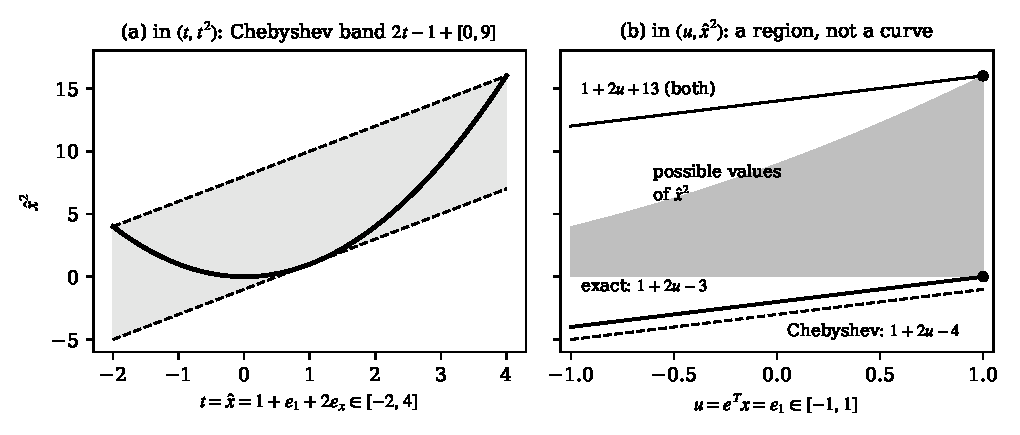
\includegraphics[width=\linewidth]{Fig2.pdf}
\caption{The square of $\hat x=1+\eps_1+2\ex$. (a) In the plane $(t,t^2)$, with $t=\hat x\in[-2,4]$, the Chebyshev band $t^2\in2t-1+[0,9]$ is the narrowest band of slope $2x_0=2$ that contains the graph. (b) The reduced form expresses $\hat x^2$ as a function of $u=\eps_1$ only, and the possible values of $\hat x^2$ form a region (gray). Both bands have slope $2$ in $u$ and share the upper line $1+2u+13$, but the lower Chebyshev line $1+2u-4$ (dashed) lies below the region, whose narrowest enclosing band has lower line $1+2u-3$ (solid).}
\label{fig:square}
\end{figure} The radius of S for a square exceeds that of SH by $\tfrac12(\|x\|_1+x_r)^2-\tfrac12x^Tx$, which approaches $\tfrac12(\|x\|_1+x_r)^2$, half the width of the exact range of the quadratic part, when the noise coefficients are spread over many symbols. Products and squares are thus two separate places where S loses with respect to the exact ranges, and in a solver both matter (Section~\ref{sec:solver}).

\paragraph{The standard multiplication is AF2 with re-centering.} An AF2 form~\cite{messine2002extentions} is
\[
\hat x = x_0+\sum_i x_i\eps_i + x_\pm\eps_\pm + x_+\eps_+ + x_-\eps_-,\qquad \eps_\pm\in[-1,1],\ \eps_+\in[0,1],\ \eps_-\in[-1,0]:
\]
besides the symmetric error term of a reduced affine form, it keeps two one-sided terms that record errors of known sign. Consider the product of two forms without one-sided terms, that is, of two reduced affine forms whose error terms $x_r\ex$ and $y_r\ey$ play the role of $x_\pm\eps_\pm$ and $y_\pm\eps_\pm$, with independent symbols. The linear part is that of~\eqref{eq:product}, and AF2 splits the nonlinear part $N$ of~\eqref{eq:N} according to the sign of its monomials. Each square $x_iy_i\eps_i^2$ ranges over $x_iy_i[0,1]$, so it has a known sign: it is added to the coefficient of $\eps_+$ when $x_iy_i>0$, and its absolute value to that of $\eps_-$ when $x_iy_i<0$, without loss. Every other monomial of $N$, that is, the bilinear terms $x_iy_j\eps_i\eps_j$ ($i\ne j$), the terms $x_ry_i\ex\eps_i$, $y_rx_i\ey\eps_i$ and $x_ry_r\ex\ey$, and the terms $x_0y_r\ey$ and $y_0x_r\ex$, ranges over an interval symmetric about $0$, and its bound, the absolute value of its coefficient, is added to the coefficient of $\eps_\pm$. This gives the product of the next proposition, which relates formula S to AF2.

\begin{propo}
\label{prop:af2}
Let $\hat x$, $\hat y$ be AF2 forms without one-sided terms, i.e., reduced affine forms whose error terms play the role of $\eps_\pm$. Their AF2 product~\cite{messine2002extentions}
\[
x_0y_0 + e^T(y_0x+x_0y) + k_1\eps_\pm + k_2\eps_+ + k_3\eps_-,\quad k_2=\sum_{x_iy_i>0}x_iy_i,\ k_3=\sum_{x_iy_i<0}|x_iy_i|,
\]
\[
k_1 = |x_0|y_r+|y_0|x_r+\sum_{i\ne j}|x_iy_j| + x_r\|y\|_1+y_r\|x\|_1+x_ry_r,
\]
becomes the product given by formula S when $k_2\eps_+$ and $k_3\eps_-$ are replaced by their centers and radii, $k_2\eps_+\in \tfrac{k_2}{2}+\tfrac{k_2}{2}[-1,1]$ and $k_3\eps_-\in-\tfrac{k_3}{2}+\tfrac{k_3}{2}[-1,1]$.
\end{propo}
\begin{proof}
The re-centered form has center shift $\tfrac12(k_2-k_3)=\tfrac12x^Ty$ and error radius $k_1+\tfrac12(k_2+k_3) = k_1+\tfrac12|x|^T|y|$, which equals $z_r$ of formula S by the identity in the proof of Proposition~\ref{prop:chain}.
\end{proof}

Thus S and AF2 have the same width after one product, and they differ only in the next operations: AF2 keeps $k_2\eps_+$ and $k_3\eps_-$, whose ranges $[0,k_2]$ and $[-k_3,0]$ are not centered at $0$, and propagates them, while S moves their midpoints to the center of the form and keeps only their radii in the symmetric error term. Among residual intervals of a given radius, a zero-centered one minimizes the width propagated through a product with another interval: if $\mathbf r=[r_c-\rho,r_c+\rho]$ and $\mathbf y$ is an interval with $Y=\max_{y\in\mathbf y}|y|$, then $\wid(\mathbf r\mathbf y)\ge 2\rho Y$, with equality for $r_c=0$. Hence S can be tighter than AF2 in compositions of products.

\begin{remark}
S can be much wider than SH even without errors: for $\hat x=\eps_1+\eps_2$ and $\hat y=\eps_1-\eps_2$, S (and AF2) give an enclosure of width $6$, while SH and E give $2$, the width of the exact range $[-1,1]$ of $\eps_1^2-\eps_2^2$.
\end{remark}

\section{Rigorous floating-point implementation}
\label{sec:rigor}

A floating-point implementation of Algorithm~\ref{alg:exact} must return an interval that contains $\rng N$. Two points need care.
\begin{itemize}
\item \emph{Angular order.} An incorrect order between two almost parallel generators would produce a path that cuts through the interior of $Z$ and could underestimate the range. The order is decided by the sign of $u_1v_2-v_1u_2$, evaluated in double precision with a forward error filter~\cite{shewchuk1997adaptive}: if $|\mathrm{fl}(u_1v_2)-\mathrm{fl}(v_1u_2)|$ exceeds $4\cdot2^{-52}(|\mathrm{fl}(u_1v_2)|+|\mathrm{fl}(v_1u_2)|)$ and neither product underflows, its sign is the exact one; otherwise the expression is evaluated in quadruple precision, where the two products are exact and the subtraction preserves the sign. Flipping a generator to the half-plane $u>0$ is exact.
\item \emph{Boundary walk.} The vertices and the values on the edges are computed in double precision, and the resulting interval is widened by an a priori bound of the rounding errors. Let $m$ be the number of generators (including $(x_r,0)$ and $(0,y_r)$ for SH), $U=|\delta_1|+3\sum_k|u_k|$ and $V=|\delta_2|+3\sum_k|v_k|$ (with $\delta=0$ for SH), which bound $|u|$ and $|v|$ at every computed or exact vertex, partial sum and edge point. Each vertex is obtained with at most $3m+2$ additions, so its error is at most $(3m+2)\,\eps_m U$ in $u$ and $(3m+2)\,\eps_m V$ in $v$, with $\eps_m=2^{-52}$, which bounds the error of one operation in any rounding mode~\cite{higham2002accuracy}. On an edge $\seg{p}{(p+d)}$ with $d=\pm2\tilde g_{(j)}$ (exact), the value at the stationary point is $P-B^2/(4A)$, with the notation above; since the stationary point is in $(0,1)$, $|B|<2|A|$, and $|P|,|A|\le UV$, $|B|\le2UV$, so each evaluated value has a rounding error of $O(\eps_m UV)$, and a wrong decision on whether the stationary point lies in $(0,1)$ changes the value by $O(\eps_m UV)$ as well. Adding the constant $\kappa$ and the term $|y_0|x_r+|x_0|y_r$ of SH, we widen the interval by $(8m+64)\,\eps_m\,(UV+|x_0|y_r+|y_0|x_r)$ and round its endpoints outwards. This widening is of the order of $10^{-13}$ times the width of the enclosure.
\end{itemize}
Our implementation sorts the generators once per product, walks the two shifted polygons of E in a single pass, and allocates no memory per product. For E, when $\min(|x_0|y_r,|y_0|x_r)=0$, it runs the single walk of SH, which gives the same interval by Corollary~\ref{cor:gain}.

For squares, both SH and E use the SH bound, that is, the Chebyshev linearization of $t^2$, which is exact when $x_r\le\|x\|_1$ (Proposition~\ref{prop:square}); the exact range of Proposition~\ref{prop:square} can be used instead at the same cost. We implemented it as an option: in 3\,000 random expressions with squares of compound subexpressions, such as $(L^2)^2$, $(L\cdot L+c)^2$ or $(\sin L+c)^2$, over random boxes, it applied in 2.5\% of the squares, those where the error of the subexpression exceeds its noise coefficients, and narrowed the enclosure by up to 25\%, without any violation of the containment test; in IbexOpt, on the medium and hard instances of the COCONUT benchmark (Section~\ref{sec:solver}), it applied only in one instance without feasible points, and it did not change the number of nodes of any instance. The center and the radius of the enclosure are then added to the reduced affine form with the usual outward rounding of the linear part.

\section{Experiments}
\label{sec:experiments}

\subsection{Range enclosures}

For these experiments, the formulae were implemented in Python, in double precision, on the representation in the variables of the introduction (a linear function of the variables plus a residual interval). The Python and C++ code of this section was written with the help of an AI assistant (see the Statements and Declarations). Univariate functions are enclosed by the same Chebyshev linearization in all methods, so that the differences come only from the products, and exact ranges were computed with IbexOpt~\cite{chabert2009}.

\paragraph{Random products.} Table~\ref{tab:random} reports single products of random forms over $[-1,1]^n$ (so that the variables are the noise symbols), with standard normal coefficients, centers of standard deviation 2, and error radii $|\mathcal N(0,1)|\rho$. Without errors ($\rho=0$), SH and E coincide, as they compute the exact range of $Q$. With errors, E is strictly narrower than SH in every product, and SH is up to 1.37 times wider than E for $n=2$; the mean advantage decreases with $n$, since the gain is bounded by $2\min(|x_0|y_r,|y_0|x_r)$ (Corollary~\ref{cor:gain}), while the width of the range of $R$, which SH computes exactly, grows with $n$. S is 1.4--2.0 times wider than E.

% table_rules_random.tex
\begin{table}[t]
\centering
\caption{Single products of random forms with $n$ variables: mean width of the enclosures of rules S and SH relative to E, and maximum of SH/E. $\rho$ scales the error radii of the operands; 500 products per row.}
\label{tab:random}
\small
\begin{tabular}{rrrrr}
\toprule
 & & \multicolumn{2}{c}{Mean width / E} & \\
\cmidrule(lr){3-4}
$n$ & $\rho$ & S & SH & max SH/E \\
\midrule
2 & 0.0 & 1.656 & 1.000 & 1.000 \\
 & 0.1 & 1.504 & 1.019 & 1.138 \\
 & 1.0 & 1.366 & 1.070 & 1.370 \\
\midrule
5 & 0.0 & 1.901 & 1.000 & 1.000 \\
 & 0.1 & 1.847 & 1.007 & 1.048 \\
 & 1.0 & 1.630 & 1.036 & 1.261 \\
\midrule
10 & 0.0 & 1.961 & 1.000 & 1.000 \\
 & 0.1 & 1.919 & 1.002 & 1.013 \\
 & 1.0 & 1.781 & 1.012 & 1.119 \\
\midrule
20 & 0.0 & 1.975 & 1.000 & 1.000 \\
 & 0.1 & 1.964 & 1.000 & 1.004 \\
 & 1.0 & 1.902 & 1.004 & 1.025 \\
\bottomrule
\end{tabular}
\end{table}

\paragraph{Test functions of Skalna and Hlad\'{\i}k.} Table~\ref{tab:sh} repeats the range-bounding experiment of~\cite[Table~3]{skalna2017new}: the nine test functions are evaluated over the same boxes, with integer powers computed as repeated products with the corresponding formula, and the overestimation $1-\wid(f^H)/\wid(\hat f)$ of the exact range $f^H$, computed with IbexOpt, is reported. For $f_1$--$f_5$, our values of S and SH agree with those of~\cite{skalna2017new} up to rounding, which validates our implementation of their formulae. For Matyas, the widths of the enclosures agree with theirs (the ratio between the widths of formulae T and S is $0.74$ in both cases), but the overestimations reported in~\cite{skalna2017new} (96--97\%) correspond to a reference range of width about 6, whereas the range of $f_7$ over $[-10,10]^2$ is $[0,100]$. For Leon, the 9\% reported for SH is below what E attains with any of the evaluation orders of the powers that we tried, so the expressions must have been evaluated in another form; the remaining differences, for $f_6$, $f_8$ and $f_9$, are presumably of the same origin.

\begin{table}[t]
\centering
\caption{Overestimation (\%) of the exact range of the test functions of~\cite{skalna2017new}, with integer powers computed as repeated products. The values of E are in bold when E is narrower than SH.}
\label{tab:sh}
\small
% table_sh.tex
\begin{tabular}{llrrr}
\toprule
Function & Box & S & SH & E \\
\midrule
$f_1$ Beale & $[-5,5]^2$ & 49.9 & 49.1 & \textbf{48.8} \\
$f_2$ Booth & $[-10,10]^2$ & 35.8 & 19.9 & 19.9 \\
$f_3$ Colville & $[-10,10]^4$ & 36.6 & 33.2 & \textbf{13.6} \\
$f_4$ Dixon ($n=5$) & $[-5,5]^5$ & 36.6 & 33.1 & \textbf{13.6} \\
$f_5$ Goldstein--Price & $[-2,2]^2$ & 99.1 & 98.6 & \textbf{98.1} \\
$f_6$ Leon & $[-1.2,1.2]^2$ & 39.1 & 28.4 & \textbf{24.4} \\
$f_7$ Matyas & $[-10,10]^2$ & 32.4 & 32.4 & 32.4 \\
$f_8$ Rosenbrock ($n=4$) & $[-5,10]^4$ & 47.5 & 36.0 & \textbf{32.3} \\
$f_9$ Six-hump camel & $[-5,5]^2$ & 57.4 & 39.9 & 39.9 \\
\bottomrule
\end{tabular}
\end{table}

E is much tighter than SH for Colville and Dixon (13.6\% instead of 33\%), and also for Leon and Rosenbrock. These functions contain squares $(x_i^2-x_j)^2$ computed as products $\hat v\cdot\hat v$ of a form that carries the error of the product $x_i\cdot x_i$ and whose center is far from zero, which is the most favorable case of Corollary~\ref{cor:gain}; in Booth and Matyas, every product has an operand without error, and E and SH coincide.


\subsection{Implementation in Ibex}
\label{sec:ibex}

We implemented SH and E in the affine arithmetic of the Ibex library~\cite{chabert2009,ibexaffine} (model fAF2 of its affine plugin), whose multiplication and square are those of formula S, with the rounding errors of each operation accumulated in the error term. Only the enclosure $[c-z_r,c+z_r]$ of $N$ (or $N_2$) changes: the linear part, its rounding errors and the way they are added to the error term are those of fAF2. Note that S is exact for the products and squares of the variables themselves, whose forms have a single noise symbol and no error, so that the formulae differ only for compound factors.

\paragraph{Validation.} The implementation was checked against the exact range of $N$ computed with rational arithmetic on 86\,000 random products, including almost parallel generators and coefficients from $10^{-6}$ to $10^6$, without any violation, and with a containment test on whole expressions: $180\,000$ random expressions from nine families that combine products, squares and $\sin$, $\cos$, $\exp$ and $\ln$ of random affine functions $L$ of the variables, such as $(L\cdot L)\cdot(L\cdot L)$, $(L\cdot L+L)^2$ or $(\sin L+L)^2\cdot(L\cdot L)$, were evaluated in affine arithmetic over random boxes with radii from $10^{-6}$ to $3$, and at sampled vertices and interior points $p$ of each box, the value $f(p)$, computed in interval arithmetic, was required to intersect the enclosure, also computed in interval arithmetic. No enclosure was violated, while the same test detects violations when the error term is artificially reduced by 10\%.

\paragraph{Cost.} Table~\ref{tab:cost} gives the time per product of the multiplication of fAF2 (S) and of SH and E. SH and E cost 2.7--5.0 times as much as S, and E costs between 0.9 and 1.1 times as much as SH in this benchmark. In the solver experiments below, this overhead is a small fraction of the time per node.

\begin{table}[t]
\centering
\caption{Time per product ($\mu$s) in the affine arithmetic of Ibex, for random forms with $n$ noise symbols, with and without error terms in the operands (C++, \texttt{-O2}, one core).}
\label{tab:cost}
\small
% table_cost.tex
\begin{tabular}{rrrrrrr}
\toprule
 & \multicolumn{3}{c}{Without errors} & \multicolumn{3}{c}{With errors} \\
\cmidrule(lr){2-4}\cmidrule(lr){5-7}
$n$ & S & SH & E & S & SH & E \\
\midrule
2 & 0.09 & 0.31 & 0.30 & 0.09 & 0.34 & 0.30 \\
5 & 0.15 & 0.41 & 0.42 & 0.16 & 0.48 & 0.42 \\
10 & 0.25 & 0.66 & 0.67 & 0.25 & 0.76 & 0.71 \\
20 & 0.47 & 1.47 & 1.61 & 0.45 & 1.59 & 1.54 \\
50 & 1.07 & 4.65 & 4.60 & 1.16 & 4.79 & 4.65 \\
100 & 2.15 & 10.56 & 10.35 & 2.13 & 10.70 & 10.61 \\
\bottomrule
\end{tabular}
\end{table}

\subsection{Global optimization with IbexOpt}
\label{sec:solver}

We replaced the multiplication and the square of fAF2 by those of SH and E in IbexOpt~\cite{chabert2009}, configured with the affine linear relaxation of~\cite{ninin2015reliable}, in which every constraint and the objective are linearized over each box by evaluating them with reduced affine forms, the lsmear bisection heuristic~\cite{araya2017}, precision $10^{-7}$ on the variables and relative precision $10^{-6}$ on the objective. All the other components of the solver are unchanged, so that the variants differ only in the enclosures of products and squares. Since the square of S is not exact for compound expressions while the Chebyshev square is a classical alternative (Proposition~\ref{prop:square}), the baseline is S$^+$: the products of S with the Chebyshev square. SH and E use the same square, so that the comparison with S$^+$ measures only the effect of the products. S, the arithmetic as distributed, is reported for reference. We used four sets of instances:
\begin{itemize}
\item \emph{synq}: 78 synthetic problems over $x\in[-1,1]^n$, $n\in\{3,5,8,10\}$. The objective is a quadratic function $x^TQx+c^Tx$ written as a sum of $n$ products of affine functions, $\sum_k(a_k^Tx)(m_k^Tx)+c^Tx$, from a factorization $Q=A^TM$ of a random symmetric matrix with a random well-conditioned $A$; the off-diagonal entries of $Q$ are nonzero with probability $\rho\in\{0.2,0.5,0.9\}$ and uniform in $[-1,1]$, and its diagonal is positive or of mixed sign. There are one linear constraint and $\lfloor n/2\rfloor-1$ constraints of the same quadratic type, made feasible by taking as right-hand side the value at a random point of the box plus a margin, and three seeds per configuration. Every product has compound factors without errors, the case where SH and E give the exact range of the nonlinear part and S does not.
\item \emph{synt}: 24 synthetic problems over $x\in[-1,1]^n$, $n\in\{3,5,8,10\}$, $\rho\in\{0.5,0.9\}$, three seeds, whose objective is a sum of $n$ terms that alternate between $(a_k^Tx)\,f_k(m_k^Tx)$ and $f_k(a_k^Tx)\,g_k(m_k^Tx)$, with $f_k,g_k\in\{\sin,\cos,\exp\}$, so that both factors of the second kind carry linearization errors; the constraints are built as for synq.
\item \emph{synp}: 18 synthetic problems over $x\in[-1,1]^n$, $n\in\{3,5,8\}$, six seeds, whose objective is $\sum_{k=1}^n q_k(x)\,r_k(x)$ plus a linear term, where each $q_k$ and $r_k$ is a random constant of absolute value in $[0.5,2]$ plus two linear terms, a square and a bilinear term, so that both factors carry errors and have nonzero centers, the favorable case of Corollary~\ref{cor:gain}; there is one random linear constraint.
\item \emph{COCONUT}: the 298 distinct instances of the optimization benchmark distributed with Ibex (sets easy, medium, hard, others, unsolved, blowup and coconutbenchmark-library2), most of them taken from the COCONUT library~\cite{coconut}. In most of them, S encloses every product as narrowly as SH and E, since S is exact on products of single variables, and the three multiplications give the same search. Table~\ref{tab:solver} reports the 110 instances in which S encloses at least one product more widely than E, as counted in a run of 5\,s with E.
\end{itemize}
Each run used one core, with four simultaneous runs on the same machine, and the time limits of Table~\ref{tab:solver}; all the variants were run in the same session, one after the other for each instance, so that their times are comparable. Table~\ref{tab:solver} reports the number of instances solved within the limit and, over the instances solved by all the variants (instances not solved by some variant are excluded from the means), the geometric means of the numbers of nodes and of the CPU times relative to S$^+$, and the comparison of E with SH. All the variants found the same optimum, within the precision, on every instance solved by all of them. Synq and synt contain no squares, so that S$^+$ coincides with S on them.

\begin{table}[t]
\centering
\caption{IbexOpt with S (the standard multiplication and square of fAF2), S$^+$ (the products of S with the Chebyshev square), SH and E (both with the Chebyshev square): instances solved within the time limit $t_{\max}$ (s), geometric means of nodes and CPU time relative to S$^+$ over the instances solved by all the variants, geometric mean of the nodes of E relative to SH, and numbers of instances where E needs at least 1\% fewer / more nodes than SH. For COCONUT, $x/y$: the $x$ instances in which S encloses some product more widely than E, out of $y$.}
\label{tab:solver}
\small
\setlength{\tabcolsep}{3.5pt}
% table_solver.tex
\begin{tabular}{lrrrrrrrrrrrrr}
\toprule
 & & & \multicolumn{4}{c}{Solved} & \multicolumn{3}{c}{Nodes / S$^+$} & \multicolumn{2}{c}{CPU / S$^+$} & \multicolumn{2}{c}{E vs SH} \\
\cmidrule(lr){4-7}\cmidrule(lr){8-10}\cmidrule(lr){11-12}\cmidrule(lr){13-14}
Set & Inst. & $t_{\max}$ & S & S$^+$ & SH & E & S & SH & E & SH & E & nodes & $<$/$>$ \\
\midrule
synq & 78 & 300 & 45 & 45 & 60 & 60 & 1.00 & 0.26 & 0.26 & 0.32 & 0.34 & 0.996 & 3/3 \\
synt & 24 & 60 & 19 & 19 & 20 & 20 & 1.00 & 0.67 & 0.62 & 0.74 & 0.69 & 0.921 & 11/1 \\
synp & 18 & 60 & 18 & 18 & 18 & 18 & 1.00 & 0.83 & 0.79 & 0.89 & 0.86 & 0.960 & 8/2 \\
COCONUT & 110/298 & 60 & 70 & 70 & 69 & 70 & 1.02 & 0.98 & 0.98 & 1.01 & 0.99 & 0.996 & 22/16 \\
\bottomrule
\end{tabular}
\end{table}

\paragraph{SH and E versus S$^+$.} On synq, SH and E solve 60 instances instead of 45 and need about four times fewer nodes (0.26) and three times less time (0.32 and 0.34) on the instances solved by S$^+$; on the 18 instances that none of them solves, the final gap between the bounds of the objective is reduced to 37\% of that of S$^+$. In synq, every product is a product of two affine forms of several variables that carry only rounding errors, so that SH and E enclose it by practically its exact range, whereas the enclosure of S is 1.7 to 2 times wider on such products (Table~\ref{tab:random}, $\rho=0$); the narrower enclosures of the objective and of the constraints give tighter linear relaxations at every node. On synt and synp, the reduction is 33\% and 17\% of the nodes. On the 110 COCONUT instances in which S loses on some product, SH and E solve practically the same instances as S$^+$ (both miss one instance that S$^+$ solves close to the time limit, and E solves one that none of the others solves within 60\,s), and need 2\% fewer nodes in the geometric mean; on the 43 instances in which S is more than 10\% wider than E on at least 10\% of the products, they need 8\% and 6\% fewer nodes than S$^+$ (over the 22 instances solved by all the variants). On the whole benchmark of 298 instances, the means of SH and E are within 3\% of those of S$^+$. The column S shows the effect of the square alone: with the square of S, the nodes grow by 3\% on the whole COCONUT benchmark, by 9\% on its medium instances, and by more than ten times on some instances, such as ex8\_4\_4bis (117\,116 nodes with S, 10\,096 with S$^+$), whose squares of compound expressions, such as $(x_i-x_j)^2$, S encloses almost twice as wide as the Chebyshev square.

\paragraph{E versus SH.} E coincides with SH on synq, where the factors carry only rounding errors, so that E and SH give practically the same enclosures (geometric mean of the nodes 0.996, with differences of more than 1\% in 6 of 45 instances, 3 in each direction), and improves on SH precisely where Corollary~\ref{cor:gain} predicts: on synt and synp, where both factors carry errors and have nonzero centers, E needs 8\% and 4\% fewer nodes than SH, and fewer nodes in 11 of 19 and 8 of 18 instances, against more in only 1 and 2. These gains are smaller than in the range enclosures of Section~\ref{sec:experiments}, because the boxes explored by the search are small and the errors carried by the factors shrink with them. On the COCONUT instances, E and SH need practically the same numbers of nodes (geometric mean 0.996; fewer in 22 instances, more in 16), and the numbers of nodes of a single instance are sensitive to tiny changes of the enclosures: in our successive implementations of SH and E, which differ only in rounding and whose enclosures differ by about $10^{-13}$ of their width, the nodes of some instances changed by a factor of more than 5. We therefore regard the differences on this set as noise.

\paragraph{Cost.} Despite the higher cost per product (Table~\ref{tab:cost}), the CPU times follow the numbers of nodes: on synt, synp and COCONUT, the times per node of SH and E are within 6\% of that of S$^+$, because the multiplication is a small part of the work at each node, dominated by the linear programs of the relaxation and by the contractors; on synq, whose objective is a sum of $n$ products of dense affine forms, they are 11\% and 24\% larger.


\section{Conclusion}

The multiplication of reduced affine forms of Skalna and Hlad\'{\i}k computes exactly the quadratic part of the product, but bounds the terms that couple the centers of the operands with their error symbols separately. Since the nonlinear part of the product is affine in each error symbol, its exact range is obtained from the ranges of shifted products over a planar zonotope at the vertices of the square of the error symbols; by central symmetry, two of them suffice, and both are computed in a single walk along the boundary, at a cost of $O(n\log n)$ operations. The resulting multiplication is the narrowest one with the usual linear part; it coincides with that of Skalna and Hlad\'{\i}k when one of the operands has no error or a zero center, and can be narrower otherwise, by at most a factor $3/2$ and by at most $2\min(|x_0|y_r,|y_0|x_r)$. Its effect on range enclosures is large on products of forms that already carry errors, such as the squares in the Colville and Dixon functions.

In an interval branch-and-bound optimizer, the main practical effect comes from computing the quadratic part exactly, which SH and E share: with respect to the standard multiplication, which is AF2 with re-centering, the number of nodes is divided by about four on problems dominated by products of compound factors, even when the standard multiplication is given the Chebyshev square; on classical benchmarks, where most products involve single variables, the square matters more than the product. The new multiplication adds a further 4--8\% where the theory predicts a gain, and coincides with SH elsewhere. Open questions are a linear-time version of Algorithm~\ref{alg:exact}, and the choice of the linear part of the product, which all the formulae considered here keep fixed.

\section*{Statements and Declarations}
\textbf{Funding.} This work was supported by the Agencia Nacional de Investigaci\'on y Desarrollo (ANID), Chile, through FONDECYT Regular project No.~1260159.
\textbf{Competing interests.} The authors have no relevant financial or non-financial interests to disclose.
\textbf{Data availability.} Code, data, the generators of the synthetic instances and the scripts that produce the tables and figures: \url{https://github.com/rilianx/exact-raf}.
\textbf{Use of AI.} The authors used an AI assistant (Claude, Anthropic) to help implement and verify the code, run the experiments and check the proofs; all code, results and proofs were reviewed by the authors, who take full responsibility for them.

\bibliographystyle{unsrt}
\bibliography{bibliography}

\end{document}
